\section{Wellen \kuchling{229} \stoecker{265}}
\subsection{Definitionen}
\begin{tabular}[]{|p{9cm}|p{9cm}|}
	\hline
	\begin{minipage}[]{9cm}
    	\textbf{Ebene harmonische Welle:}\\
 		$\xi(\vec{r},t)=\xi_0 \sin(\omega t -k\vec{r}+\varphi)$\\ \\		   	
 		$\xi(\vec{r},t)=\xi_0 e^{-j(\omega t-k\vec{r})}$\\ \\ 
 		\textbf{Harmonische Kugelwelle:}\\
 		$\xi(\vec{r},t)=\dfrac{\xi_0}{|\vec{r}|} \sin(\omega
 		t-k|\vec{r}|+\varphi)$\\\\
 		$\xi(\vec{r},t)=\dfrac{\xi_0}{|\vec{r}|} e^{-j(\omega t-k|\vec{r}|)}$\\ 		
    \end{minipage} &
	\begin{minipage}[]{9cm}
    	\vspace{0.2cm}    
    	$\xi({\vec{r},t})$ = Auslenkung am Ort $\vec{r}$ zur Zeit $t$\\
		$\xi_0$ = Amplitude $[1]$\\
		$k$ = Wellenzahl $[\frac{1}{m}]$\\
		$\vec{r}$ = Ortsvektor $[m]$\\
		$\omega$ = Kreisfrequenz $[\frac{1}{s}]$\\
		$\varphi$ = Phasenverschiebung $[rad]$\\    
		$\lambda$ = Wellenlänge $[m]$\\
		$u$ = Wellengeschwindigkeit $[\frac{m}{s}]$\\
		$f$ = Frequenz $[Hz]$\\
		$T$ = Periodendauer $[s]$\\
    \end{minipage} \\
	\hline
\end{tabular}

\subsection{Wichtige Beziehungen}
$\boxed{k=\dfrac{\omega}{u}=\dfrac{2\pi}{\lambda}}$\quad
$\boxed{u=\dfrac{\omega}{k}}$ \quad
$\boxed{\lambda=\dfrac{2\pi}{k}=\dfrac{u}{f}}$ \quad
$\boxed{\omega=2\pi f=\dfrac{2\pi}{T}}$ \quad
$\boxed{f=\dfrac{\omega}{2\pi}=\dfrac{u}{\lambda}=\dfrac{1}{T}}$ \quad
$\boxed{T=\dfrac{1}{f}=\dfrac{2\pi}{\omega}}$ \quad
$\boxed{\varphi=\omega t-k|\vec{r}|}$

\subsection{Wellengeschwindigkeit \kuchling{233} \stoecker{267}}
\renewcommand{\arraystretch}{1.5}
\begin{tabular}{| p{6cm} | p{6cm} | p{6cm} |}
\hline
\textbf{Elastisch}e L"angs-/ Longitudinalwelle & \textbf{Elastisch}e Quer-/ Transversalwelle & Transversalwellen bei \textbf{Saite} oder Seil\\
$u=\sqrt{\dfrac{E}{\varrho}}$ & $u=\sqrt{\dfrac{G}{\varrho}}$ &
$u=\sqrt{\dfrac{F}{\varrho\,A}}=\sqrt{\dfrac{F}{\varrho}+\dfrac{\pi\,E\,A}{\varrho\,\lambda^2}}$
\\ $E$: Elastizit"atsmodul& $G$: Schubmodul & $F$: Spannkraft, $E$:
Elastizit"atsmodul \\
\hline

Schwerewellen in \textbf{tiefem Wasser} & Schwerewellen in \textbf{flachem Wasser}& \textbf{Kapillarwellen}\\
$u=\sqrt{\dfrac{g\,\lambda}{2\pi}}$&$u=\sqrt{g\,h}$&$u=\sqrt{\dfrac{2\pi\,\sigma}{\varrho\,\lambda}}$\\
($\lambda \ll h$) & ($\lambda \gg h$)  & $\sigma$: Oberfl"achenspannung \\
\hline

Schallwellen in \textbf{Fluide}n & Schallwellen in \textbf{Gas}en & $M_{Luft}=
0.02883 \dfrac{kg}{mol} = 28.83 \dfrac{g}{mol}$\\
$u=\sqrt{\dfrac{1}{\varrho\,\kappa}}$&$u=\sqrt{\dfrac{\varkappa\,p}{\varrho}}=\sqrt{\dfrac{\varkappa\,R\,T}{M}}$&$R=8.3145 \dfrac{J}{mol\cdot K}$\\
$\kappa$: Kompressibilit"at &$p$: Druck, $M$: Molmasse&$\varkappa_{Luft}=1.4$\\
& $\varkappa$: Adiabatenexponent&$\text{T:
}C^\circ+273,15K$\\
\hline
\end{tabular}
\renewcommand{\arraystretch}{1}

\subsection{Eigenschwingungen \kuchling{334} \stoecker{294}}
\renewcommand{\arraystretch}{2.7}
\begin{tabular}{|l|llll|}
\hline
\textbf{Saiten}
	& Grundfrequenz: 
	& $ f_1=\dfrac{1}{2l}\sqrt{\dfrac{F}{\varrho\,A}}$
	& Oberschwingungen: $ f_n=n\, f_1$
	& $\lambda_n=\dfrac{2l}{n}$\\
\hline
\textbf{Pfeifen} & Offen:
 	& $f_1=\dfrac{1}{2l}\,u_{\text{Gas}}=\dfrac{1}{2l}\sqrt{\dfrac{\varkappa\,R\,T}{M}}$ 
	& $f_n=n\, f_1$
	& $\lambda_n=\dfrac{4l}{n}$ \quad ($n=1,3,5,...$) \\
& Gedackt: 
 	& $ f_1=\dfrac{1}{4l}\sqrt{\dfrac{\varkappa\,R\,T}{M}}$
	& $f_n=(2n+1) f_1$
	& $\lambda_n=\dfrac{4l}{n}$ \quad ($n=2,4,6,...$) \\ 
\hline
\textbf{Membranen}
 	& &
 	$f_{mn}=\dfrac{1}{2}\sqrt{\dfrac{F}{\mu}}\sqrt{\dfrac{m^2}{a^2}+\dfrac{n^2}{b}}$ 
	& \multicolumn{2}{l|}{\parbox{8cm}{$m,n$: Anz. Oberwellen und $a,b$:
	L"ange/Breite \\
	$\mu$: Masse / Fläche; $F$: Spannkraft / Länge}} \\ \hline
\end{tabular}
\newpage

\subsection{Doppler-Effekt \kuchling{342} \stoecker{277}}
\begin{tabular}{|l|l|l|}
\hline
\begin{minipage}[]{4cm}
		\small
		\vspace{.2cm}
		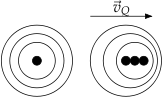
\includegraphics[width=3cm]{./bilder/doppler.png}\\
		Ruhende \& bewegte Punktquelle \\ \\ \\
		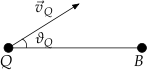
\includegraphics[width=3cm]{./bilder/doppler-bewegte-quelle.png}\\
		Bewegte Punktquelle \\ \\ \\
		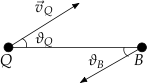
\includegraphics[width=3cm]{./bilder/doppler-beide-bewegt.png} \\
		Bewegter Beobachter \& bewegte Quelle \\
		\end{minipage}
	& \begin{minipage}[]{7cm}
      	\renewcommand{\arraystretch}{2}
      	\vspace{.2cm}
	  	\textbf{Bewegte Quelle, ruhender Beobachter} \\
	  	$f_B = \dfrac{1}{1 \mp  \dfrac{v_Q}{u}} f_Q$ \qquad - auf Hörer zu \\
	  	$f_B = \dfrac{1}{1 - \dfrac{v_Q}{u} \cos(\vartheta_Q)} f_Q$ \\
	  	\vspace{.5cm}\\
	  	\textbf{Ruhende Quelle, bewegter Beobachter} \\
	  	$f_B = \left(1 \pm \dfrac{v_B}{u}\right) f_Q$ \qquad + auf Quelle zu \\
	  	$f_B = \left(1 + \dfrac{v_B}{u} \cos(\vartheta_B)\right) f_Q$ \\
	  	\vspace{.5cm}\\
	  	\textbf{Allgemein} \\
	  	$f_B = \dfrac{u + v_B \cos(v_B)}{u - v_Q \cos(v_Q)} f_Q$ \\
	  	\vspace{.5cm}\\
	  	\textbf{Optischer (transversaler) Dop.-Effekt } \\
	  	$f_B = \dfrac{\sqrt{1 - \beta^2}}{1 - \beta \cos \vartheta_{rel}} f_Q \qquad \beta =
	  	\dfrac{v_{rel}}{c}$ \\ \vspace{.5cm}\\
	  	\textbf{Schwebungsfrequenz}\\
	  	$\Delta f = |f_{Empfangen} - f_{Gesendet}|$ \\ \vspace{.2cm}
      	\renewcommand{\arraystretch}{1}
    	\end{minipage}
	& \parbox{6.5cm}{
		$f_B \;$ gehörte Frequenz \\
		$f_Q \;$ gesendete Frequenz \\
		$v_B \;$ Geschwindigkeit Beobachter \\
		$v_Q \;$ Geschwindigkeit Quelle\\
		$v_{rel} \;$ Relativgeschwindigkeit zwischen Quelle und Beobachter\\
		$\vartheta_{rel} \;$ Winkel zwischen $\vec{v}_{rel}$ und $\overline{BQ}$\\
		$u \;$ Phasengeschw., meist $u = c_0 \approx 3 \cdot 10^8 \frac{m}{s}$
		} \\
\hline
\end{tabular}

\subsection{Machscher Kegel \kuchling{344} \stoecker{278}}
\begin{tabular}{ll}
\parbox{5cm}{
	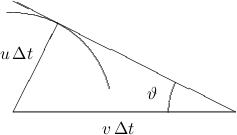
\includegraphics[width=4cm]{./bilder/machscher-kegel.png}}
	& $\sin(\vartheta)=\dfrac{u}{v}$ \qquad \qquad Machzahl: $M=\dfrac{v}{u}$
\end{tabular}

\subsection{Optische Länge}
Durchqueren Wellen Medien, muss mit optischen Längen gerechnet werden.\qquad 
$s$ wird zu $n\,s$ \qquad $\lambda$ wird zu $\dfrac{\lambda}{n}$



\subsection{"Uberlagerung / Interferenz \kuchling{233, 235} \stoecker{272, 354}}
\setlength{\tabcolsep}{5pt}
\renewcommand{\arraystretch}{2}
\subsubsection{Interferenzbedingungen}
\begin{tabular}{p{11cm} p{7cm}}
\begin{minipage}[]{11cm}
	\begin{tabular}{|l|l|l|}
	\hline
	& \textbf{Phase} & \textbf{Weg} \\
	\hline
	Konstruktiv: 
		& $k_1\cdot r_1-k_2\cdot r_2=m \, 2\pi$
		& $n \, \Delta r \, \frac{\lambda}{2} = m \, \lambda$ \\
	Destruktiv: 
	 	& $k_1\cdot r_1-k_2\cdot r_2=(2m+1)\pi$
	 	& $n \, \Delta r \, \frac{\lambda}{2} = (2m+1) \frac{\lambda}{2}$ \\
	\hline
	\end{tabular}\\
	\end{minipage}

	& \parbox{7cm}{
		Ein Phasensprung um $\pi$ bzw. $\frac{\lambda}{2}$ findet bei
		\textbf{Reflektion} an einem härteren oder optisch dichterem Material
		(\textbf{höheres $n$}) statt.
	}
\end{tabular}
\newpage

\section{Akustik \kuchling{333} \stoecker{287}}
\setlength{\tabcolsep}{5pt}
\renewcommand{\arraystretch}{2.5}
\begin{tabular}{ll}
Welle: & $\xi=\xi_0\sin(\omega t-kx)$ \qquad $\xi_0$ Schallausschlag \\
Schallschnelle: & $v=v_0\cos(\omega t-kx)\qquad\rightarrow\qquad v=\dot{\xi}=\omega\xi_0\cos(\omega t-kx)\rightarrow \dfrac{v_0}{\omega}=\xi_0$\\
Schalldruck: & $\tilde p=\Delta p \cos(\omega t-kx)$ \\
Druckamplitude: & $\Delta p_0=Z\cdot v_0$ \qquad Schallimpedanz $Z=\varrho
\cdot u$\\ Schallintensit"at: & $I=\dfrac{1}{2}\,\varrho\, v_0^{\,2}\,u =
\dfrac{1}{2}\varrho\,\omega^2\, \xi_0^{\,2}\,u =  \dfrac{\Delta
p_0^{\,2}}{2\cdot Z}$ \qquad $\xi_0$ Schallausschlag; $\varrho$ Dichte des Mediums\\  

Schallintensit"atspegel: & $L_I=10\cdot \log\left(\dfrac{I}{I_0}\right)$\qquad $I_0=10^{-12}$ W/m$^2$ \qquad $L_I=L_p$ f"ur Z=400kg/m$^2$s @ 20$^{\circ}$C\\
Schalldruckpegel: & $L_p=20\cdot\log\left(\dfrac{p_{\text{eff}}}{p_{\text{eff}_0}}\right)= 20\cdot\log\left(\dfrac{\tilde p}{\sqrt{2}\cdot p_{\text{eff}_0}}\right)$\qquad $p_{\text{eff}_0}=2\cdot 10^{-5}$ Pa\\
Schallschnellenpegel: & $L_v=20\cdot\log\left(\dfrac{v_{\text{eff}}}{v_{\text{eff}_0}}\right)$ \qquad $v_{\text{eff}_0}=5\cdot10^{-8}$m/s \\
Schallleistungspegel: & $10\cdot\log\left(\dfrac{P}{P_0}\right)$ \qquad $P_0=10^{-12}$W\\
Schallfluss: & $\vec q=\int\limits_{A}{\vec v\cdot dA}$\\
Wellengeschwindigkeit: & $u=\sqrt{\dfrac{1}{\varrho\,\kappa}}=\underbrace{\sqrt{\dfrac{\varkappa\,p}{\varrho}}=\sqrt{\dfrac{\varkappa\,R\,T}{M}}}_{\text{f"ur Gase}}$ \qquad (Schallgeschwindigkeit) $\kappa$: Kompressibilit"at \quad\\
& $\Rightarrow\dfrac{\Delta V}{V}=-\kappa\cdot\Delta p$ \qquad ($p\cdot V=\text{const}\,\,@\,\,T_{\text{const}}$ bzw. $p\cdot V^{\varkappa}=\text{const}$) \\
Lautheit: & $S=2^{0.1\cdot(L_S-40)}$ \qquad $L_S=$ Lautst"arkepegel [phon] = $L_P$ @ 1kHz, H"orschwelle 4phon\\
Kugelwellen: & (Punktquellen) $I=\dfrac{P}{4\pi r^2}\quad\rightarrow\quad \sim\dfrac{1}{r^2}$ und $\dfrac{I_2}{I_1}=\dfrac{r_1^{\,2}}{r_2^{\,2}}$  \\
& $\Delta L_I=L_{I_1}-L_{I_2}=20\cdot\log\left(\dfrac{r_2}{r_1}\right)$ \\
& Luftd"ampfung: $K$ [dB/m] $\Rightarrow$ $L_2=L_1-\underbrace{20\cdot\log\left(\dfrac{r_2}{r_1}\right)}_{\text{geom. D"ampfung}}-\underbrace{K\cdot(r_2-r_1)}_{\text{Luftd"ampfung}}$\quad $K$: D"ampfung [dB/m]\\
Zylinderwellen: & (Linienquellen) $I=\dfrac{P}{l\,2\pi r}\quad\rightarrow\quad \sim\dfrac{1}{r} \quad \Rightarrow L_2=L_1-10\cdot\log\left(\dfrac{r_2}{r_1}\right)-K\cdot(r_2-r_1)$ \\
Ebene Welle & (z.B. Parabolspiegel) $\rightarrow$ konstantes I, keine geom. D"ampfung nur Luftd"ampfung\\
& $L_2=L_1-K\cdot(r_2-r_1)$ f"ur $d<<r\quad\rightarrow\quad$ $I_2=\dfrac{P}{4\pi(r+d)^2}\approx\dfrac{P}{4\pi r^2}=I_2$\quad$I=$const\\
Schalld"ammung: & $R=10\,\log\left(\dfrac{P_1}{P_2}\right)$ \\
Phasensprung & bei Reflexion w"ahrend "Ubergang von gasf"ormig $\rightarrow$ fest  \\
Infra-/Ultraschall & Infraschall $<$ 16Hz...20kHz $<$ Ultraschall ...10GHz $<$ Hyperschall\\
\end{tabular}
